\documentclass[12pt]{article}
\usepackage[spanish,es-nodecimaldot]{babel}
\usepackage[utf8]{inputenc}
\usepackage[T1]{fontenc}
\usepackage[a4paper,margin=2.5cm]{geometry}
\usepackage{lmodern}
\usepackage{setspace}
\usepackage{parskip}
\usepackage{graphicx}
\usepackage{float}
\usepackage{amsmath}

\begin{document}
\thispagestyle{empty}

\begin{center}
    \textsc{Universidad Central de Venezuela}\\[0.35cm]
    \textsc{Facultad de Ingenier\'ia}\\[0.35cm]
    \textsc{Escuela de Ingenier\'ia El\'ectrica}\\[0.35cm]
    \textsc{Departamento de Potencia}\\[0.35cm]
    \textsc{Laboratorio de M\'aquinas El\'ectricas I}
\end{center}

\vspace{6.8cm}

\begin{center}
    \textbf{PRE-LABORATORIO N\textsuperscript{o} 6}\\[0.35cm]
    \textbf{Transformador monof\'asico. Rendimiento}
\end{center}

\vfill

\noindent
\begin{minipage}[t]{0.48\textwidth}
    Docente:\\[0.25cm]
    Jes\'us Blondel
\end{minipage}%
\hfill
\begin{minipage}[t]{0.48\textwidth}
    \raggedleft
    Autor:\\[0.25cm]
    Br. Carla Fajardo\\[0.25cm]
    V-27.571.576
\end{minipage}

\vspace{1.1cm}

\begin{center}
    Caracas, \today
\end{center}

\newpage

\section{Introducci\'on}
El transformador monof\'asico es un equipo fundamental en los sistemas el\'ectricos, ya que permite transferir energ\'ia entre circuitos de corriente alterna y adaptar los niveles de tensi\'on y corriente. Para evaluar su funcionamiento no basta con conocer sus valores nominales: tambi\'en es necesario observar c\'omo responde ante distintas condiciones de carga y qu\'e proporci\'on de la potencia de entrada se entrega efectivamente a la carga.

En el siguiente prelaboratorio se estudia el rendimiento del transformador monof\'asico al operar con cargas resistivas e inductivas. Se consideran la influencia del factor de potencia y las p\'erdidas en el hierro y en los devanados, as\'i como la condici\'on te\'orica de m\'aximo rendimiento. Estos conceptos permiten interpretar las curvas de rendimiento y relacionar la potencia suministrada con la potencia absorbida.

\newpage

\section{Objetivos}

\subsection*{Objetivo general}
Observar y analizar el comportamiento del rendimiento de un transformador monofásico

\subsection*{Objetivos espec\'ificos}
\begin{itemize}
    \item Medir la curva de rendimiento del transformador para una carga resistiva.
    \item Determinar, para el punto a plena carga, la temperatura del ensayo por el método de la resistencia.
    \item Medir un punto del rendimiento del transformador para una carga inductiva.
\end{itemize}
\newpage

\section{Marco te\'orico}
\subsection{Introducci\'on al transformador monof\'asico}

El transformador monof\'asico es una m\'aquina el\'ectrica est\'atica que transfiere energ\'ia el\'ectrica entre dos o m\'as circuitos mediante la acci\'on de un campo magn\'etico variable, modificando los niveles de tensi\'on y corriente pero manteniendo constante la frecuencia ($f_1 = f_2$). Consta esencialmente de dos devanados el\'ectricos (el primario, conectado a la fuente de alimentaci\'on, y el secundario, conectado a la carga) arrollados sobre un n\'ucleo magn\'etico cerrado. Este n\'ucleo est\'a construido mediante el apilamiento de chapas o l\'aminas de acero al silicio aisladas entre s\'i, dise\~nado para minimizar las p\'erdidas de energ\'ia por corrientes par\'asitas e hist\'eresis.

\subsection{P\'erdidas y rendimiento}
El rendimiento de un transformador ($\eta$) se expresa como el cociente entre la potencia \''util entregada a la carga ($P_2$) y la potencia activa absorbida en la entrada ($P_1$):
\begin{equation}
    \eta = \frac{P_2}{P_1}
    = \frac{P_2}{P_2 + P_p}
    = \frac{C S_N \cos\varphi_2}{C S_N \cos\varphi_2 + P_{Fe} + C^2 P_{Cu,N}}
\end{equation}

Las p\'erdidas totales ($P_p$) se dividen en dos grupos principales:
\begin{enumerate}
    \item \textbf{P\'erdidas fijas o p\'erdidas en el hierro ($P_{Fe}$):} producidas en el n\'ucleo magn\'etico por el fen\'omeno de hist\'eresis y las corrientes par\'asitas o de Foucault. Dependen de la tensi\'on y la frecuencia aplicadas y permanecen pr\'acticamente constantes para cualquier nivel de carga.
    \item \textbf{P\'erdidas variables o p\'erdidas en el cobre ($P_{Cu}$):} ocasionadas por el calentamiento resistivo ($I^2R$) en los devanados. Var\'ian proporcionalmente al cuadrado del \`indice de carga ($C = S/S_N = I_2/I_{2N}$), cumpli\'endose que $P_{Cu} = C^2 P_{Cu,N}$.
\end{enumerate}

\subsection{Rendimiento m\'aximo}
El rendimiento de un transformador var\'ia en funci\'on de la potencia demandada por la carga. Matem\'aticamente, al derivar la funci\'on de rendimiento respecto al \`indice de carga ($d\eta/dC = 0$), se obtiene la condici\'on de rendimiento m\'aximo:
\begin{equation}
    P_{Fe} = P_{Cu} = C^2 P_{Cu,N}
\end{equation}

Es decir, el rendimiento alcanza su valor \'optimo en el punto de operaci\'on donde las p\'erdidas fijas en el hierro igualan a las p\'erdidas variables en el cobre.
\begin{itemize}
    \item \textbf{\'Indice de carga \'optimo ($C_{\text{opt}}$):}
    \begin{equation}
        C_{\text{opt}} = \sqrt{\frac{P_{Fe}}{P_{Cu,N}}}
    \end{equation}
    \item \textbf{Potencia aparente de m\'aximo rendimiento:}
    \begin{equation}
        S_{\text{max}} = C_{\text{opt}} \cdot S_N
        = S_N \sqrt{\frac{P_{Fe}}{P_{Cu,N}}}
    \end{equation}
    \item \textbf{Criterio de dise\~no:} los transformadores de potencia se dise\~nan para tener su punto \'optimo entre el 50\% y el 70\% de su capacidad nominal ($C_{\text{opt}} \approx 0.5$--$0.7$), mientras que en transformadores de distribuci\'on se dise\~na entre el 30\% y el 50\% para optimizar la eficiencia energ\'etica promedio a cargas reducidas.
\end{itemize}

\subsection{Determinaci\'on de temperatura por el m\'etodo de la resistencia}
La vida \'util del aislamiento de un transformador depende cr\'iticamente de la temperatura de operaci\'on en sus devanados. Seg\'un la ley de Montsinger, un aumento continuo de $10\,^{\circ}\mathrm{C}$ reduce la vida del aislante a la mitad.

Dado que es dif\'icil colocar term\'ometros directamente en el punto m\'as caliente del devanado sumergido, se recurre al m\'etodo indirecto de medici\'on de resistencia en corriente continua:
\begin{enumerate}
    \item \textbf{Medici\'on en fr\'io:} se mide la resistencia \'ohmica del devanado ($R_1$) a una temperatura ambiente conocida ($T_1$), antes de energizar la m\'aquina.
    \item \textbf{Prueba de calentamiento:} el transformador opera bajo carga hasta alcanzar la temperatura de r\'egimen permanente.
    \item \textbf{Medici\'on en caliente:} se desconecta la m\'aquina y se mide r\'apidamente la nueva resistencia del devanado ($R_2$).
    \item \textbf{Ecuaci\'on de temperatura:} aprovechando la variaci\'on lineal de la resistencia del conductor con la temperatura, la temperatura final ($T_2$) se calcula mediante:
    \begin{equation}
        \frac{R_2}{R_1} = \frac{T_2 + T_k}{T_1 + T_k}
        \quad\Longrightarrow\quad
        T_2 = \frac{R_2}{R_1}(T_1 + T_k) - T_k
    \end{equation}
\end{enumerate}

La elevaci\'on de temperatura del devanado es $\Delta T = T_2 - T_1$. En estas expresiones, $T_k = 234.5\,^{\circ}\mathrm{C}$ para conductores de cobre y $T_k = 225\,^{\circ}\mathrm{C}$ para conductores de aluminio.
\newpage

\section{Trabajo previo}
Predeterminar la curva de rendimiento del transformador para una carga resistiva y una carga inductiva.

\begin{figure}[H]
    \centering
    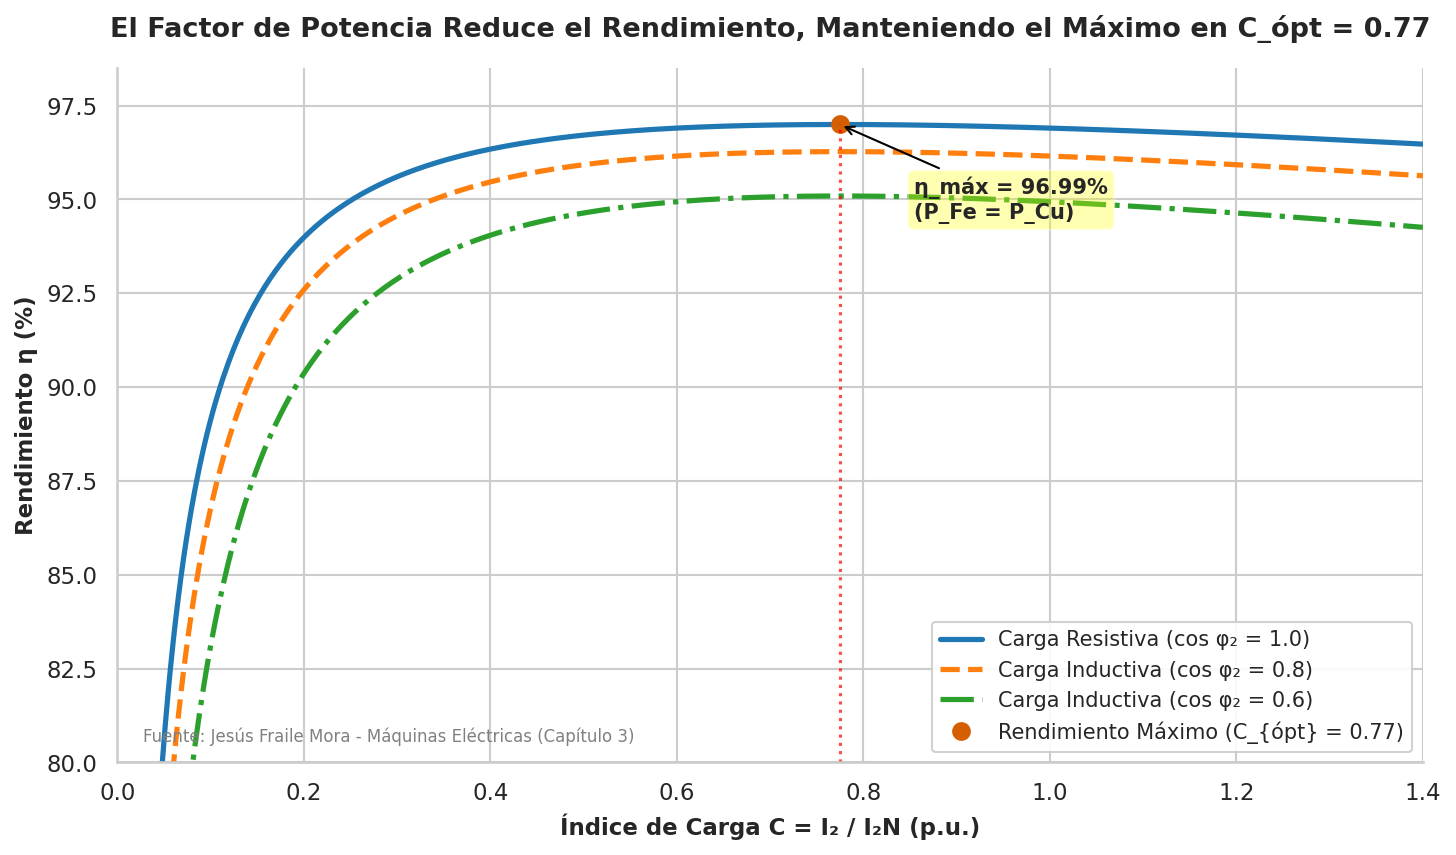
\includegraphics[width=0.95\textwidth]{imagenes/curvas_rendimiento_transformador.png}
    \caption{Curvas de rendimiento del transformador para carga resistiva y capacitiva para distintos factores de potencia}
    \label{fig:curvas-rendimiento-transformador}
\end{figure}

\begin{itemize}
    \item \textbf{L\'inea azul (carga resistiva, $\cos\varphi_2 = 1.0$):} Para una misma corriente de carga, el rendimiento es m\'aximo cuando la carga es puramente resistiva y no existe desfase entre la tensi\'on y la corriente.
    \item \textbf{L\'inea naranja (carga inductiva, $\cos\varphi_2 = 0.8$):} Muestra un rendimiento menor que la carga resistiva. Un factor de potencia menor reduce la potencia activa de salida para una misma potencia aparente y puede aumentar la corriente y las p\'erdidas en los devanados.
    \item \textbf{L\'inea verde (carga inductiva, $\cos\varphi_2 = 0.6$):} Un factor de potencia m\'as bajo reduce a\'un m\'as el rendimiento de la m\'aquina.
\end{itemize}

Se puede decir que a medida que el factor de potencia disminuye de 1.0 a 0.6, la curva de rendimiento se desplaza hacia abajo, lo cual es un resultado completamente esperado ya que el factor de potencia reduce el rendimiento
ya que un factor de potencia bajo obliga a la máquina a hacer circular más corriente para entregar la misma potencia útil. Este esfuerzo extra se traduce en más calor, es decir, en pérdidas, lo que reduce la relación entre lo que sale y lo que entra, por lo que se reduce el rendimiento.

\newpage

\section{Equipos e instrumentos}
\begin{table}[H]
\centering
\begin{tabular}{|c|}
\hline
Transformador monofásico \\ \hline
Variac (Autotransformador variable) \\ \hline
Voltímetro de hierro móvil \\ \hline
Amperímetro de hierro móvil \\ \hline
Vatímetro \\ \hline
Fuente de alimentación AC \\ \hline
Fuente de alimentación DC \\ \hline
Reostato \\ \hline
Carga \\ \hline
Cables de conexión \\ \hline
Interruptor de prueba \\ \hline
\end{tabular}
\caption{Equipos e instrumentos de laboratorio.}
\end{table}

\section{Diagramas de conexi\'on}

\begin{figure}[H]
    \centering
    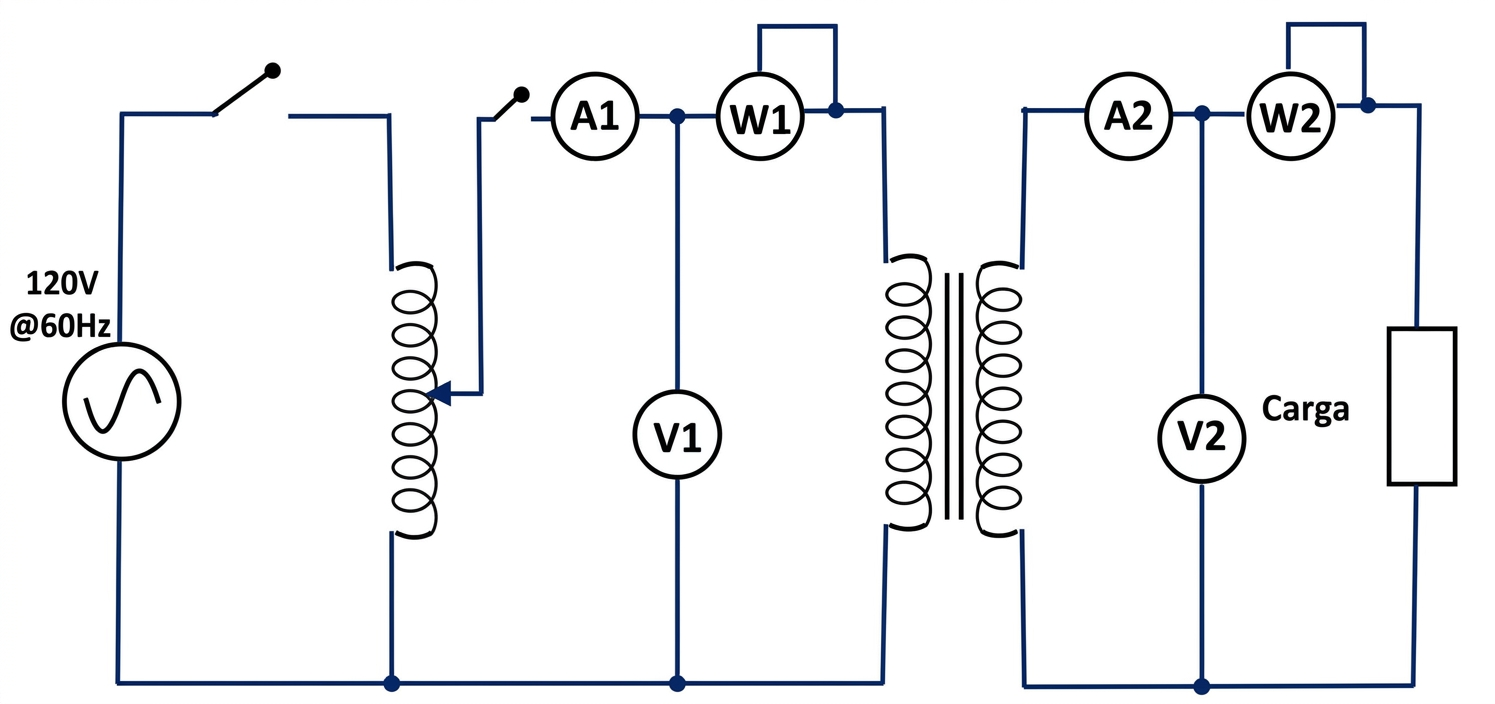
\includegraphics[width=0.7\textwidth]{imagenes/dia1.jpg}
    \caption{Conexi\'on para la evaluaci\'on del rendimiento del transformador monof\'asico.}
    \label{fig:diagrama-conexion-transformador}
\end{figure}

\begin{figure}[H]
    \centering
    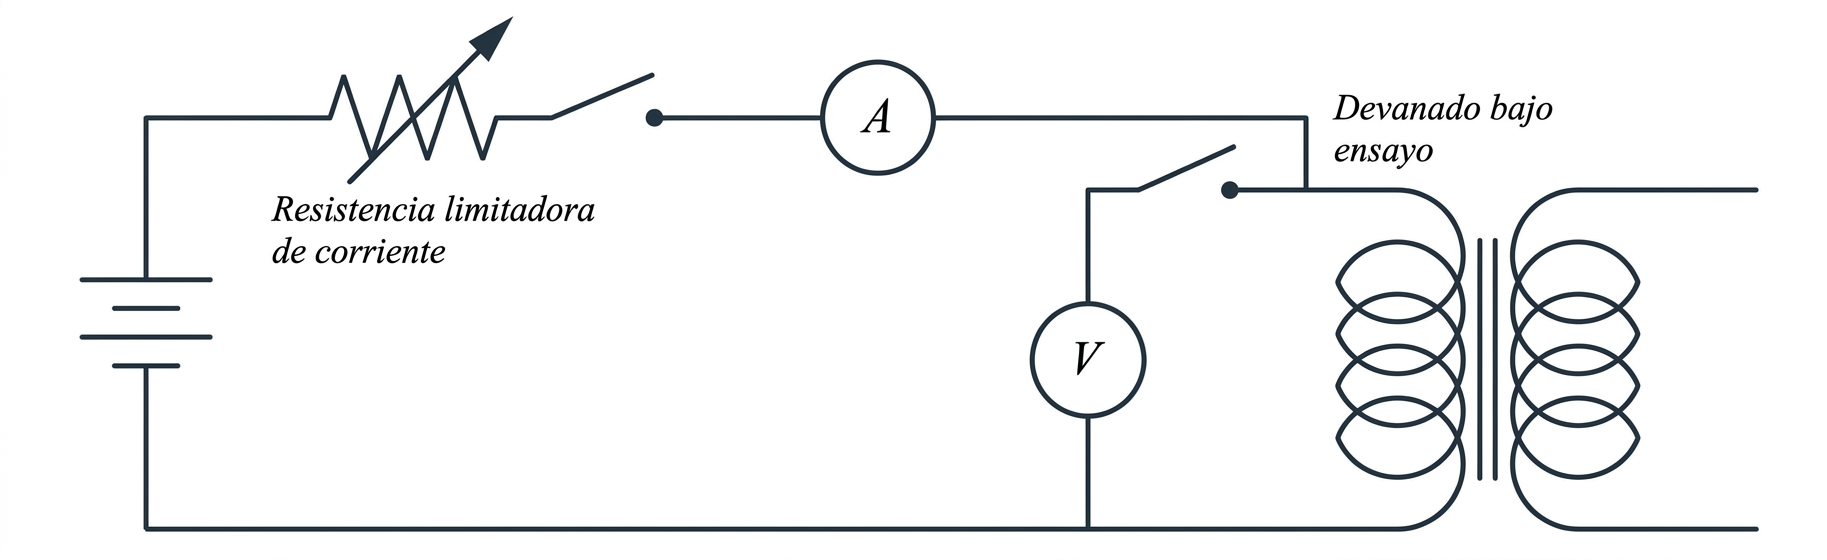
\includegraphics[width=0.9\textwidth]{imagenes/dia2.jpg}
    \caption{M\'etodo del Volt\'imetro - Amper\'imetro}
    \label{fig:diagrama-conexion-12}
\end{figure}

\section{Metodolog\'ia}

\subsection*{Metodolog\'ia espec\'ifica de la Pr\'actica 6: Transformador Monof\'asico. Rendimiento}
\begin{enumerate}
    \item \textbf{Obtener previamente la informaci\'on t\'ecnica del transformador} a utilizar:
    \begin{itemize}
        \item Caracter\'isticas el\'ectricas.
        \item Datos de placa.
        \item Condiciones nominales.
    \end{itemize}
    \item \textbf{Conectar el circuito} a trav\'es del VARIAC y el breaker, solicitando autorizaci\'on al profesor para energizar.
    \item \textbf{Medir la resistencia de los devanados}:
    \begin{itemize}
        \item Con el m\'etodo del volt\'imetro - amper\'imetro se procede a medir la resistencia de cada devanado del transformador.
        \item Se registran las mediciones.
        \item Luego al finalizar cada ensayo, es decir, el ensayo de carga resistiva y carga inductiva se procede a medir nuevamente la resistencia de cada devanado del transformador.
        \item Se registran las mediciones para as\'i poder obtener la temperatura de operaci\'on.
    \end{itemize}
    \item \textbf{Rendimiento del transformador para una carga resistiva e inductiva}:
    \begin{itemize} 
        \item Se procede a conectar una carga resistiva al devanado secundario del transformador.
        \item Luego se alimenta el transformador por el lado de alta y se lleva a su valor nominal.
        \item Se procede a variar la carga resistiva al menos hasta la plena carga nominal y se registran los valores de voltaje, corriente y potencia en ambos lados del transformador.
        \item Luego se conecta una carga inductiva al devanado secundario del transformador.
        \item Se procede a seguir el mismo procedimiento que para la carga resistiva, variando la carga inductiva al menos hasta la plena carga nominal y registrando los valores de voltaje, corriente y potencia en ambos lados del transformador.
    \end{itemize}
\end{enumerate}
\newpage

\section{Tabla de Resultados}

\begin{table}[H]
\centering
\caption{Resultados experimentales para el ensayo con carga resistiva.}
\resizebox{\textwidth}{!}{%
\begin{tabular}{|c|c|c|c|c|c|c|c|}
\hline
\textbf{Carga (W)} & $V_1$ (V) & $I_1$ (A) & $P_1$ (W) & $V_2$ (V) & $I_2$ (A) & $P_2$ (W) & \textbf{Rendimiento (\%)} \\ \hline
\rule{0pt}{0.8cm} & & & & & & & \\ \hline
\rule{0pt}{0.8cm} & & & & & & & \\ \hline
\rule{0pt}{0.8cm} & & & & & & & \\ \hline
\rule{0pt}{0.8cm} & & & & & & & \\ \hline
\rule{0pt}{0.8cm} & & & & & & & \\ \hline
\rule{0pt}{0.8cm} & & & & & & & \\ \hline
\rule{0pt}{0.8cm} & & & & & & & \\ \hline
\rule{0pt}{0.8cm} & & & & & & & \\ \hline
\rule{0pt}{0.8cm} & & & & & & & \\ \hline
\rule{0pt}{0.8cm} & & & & & & & \\ \hline
\end{tabular}%
}
\end{table}

\begin{table}[H]
\centering
\caption{Resultados experimentales para el ensayo con carga inductiva.}
\resizebox{\textwidth}{!}{%
\begin{tabular}{|c|c|c|c|c|c|c|c|}
\hline
\textbf{Carga (W)} & $V_1$ (V) & $I_1$ (A) & $P_1$ (W) & $V_2$ (V) & $I_2$ (A) & $P_2$ (W) & \textbf{Rendimiento (\%)} \\ \hline
\rule{0pt}{0.8cm} & & & & & & & \\ \hline
\rule{0pt}{0.8cm} & & & & & & & \\ \hline
\rule{0pt}{0.8cm} & & & & & & & \\ \hline
\rule{0pt}{0.8cm} & & & & & & & \\ \hline
\rule{0pt}{0.8cm} & & & & & & & \\ \hline
\rule{0pt}{0.8cm} & & & & & & & \\ \hline
\rule{0pt}{0.8cm} & & & & & & & \\ \hline
\rule{0pt}{0.8cm} & & & & & & & \\ \hline
\rule{0pt}{0.8cm} & & & & & & & \\ \hline
\rule{0pt}{0.8cm} & & & & & & & \\ \hline
\end{tabular}%
}
\end{table}

\newpage

\section{Referencias}
\begin{enumerate}
    \item Nerio Ojeda, Juli\'an P\'erez. \textit{Pr\'actica 6. Transformador Monof\'asico. Rendimiento}. Universidad Central de Venezuela, Facultad de Ingenier\'ia, Escuela de Ingenier\'ia El\'ectrica, Departamento de Potencia, Laboratorio de M\'aquinas I, Revisi\'on 201.
    \item Fraile Mora, Jes\'us. \textit{M\'aquinas El\'ectricas} (6.\textsuperscript{a} ed.). McGraw-Hill, 2008.
\end{enumerate}

\end{document}